% !TEX program = xelatex
\documentclass[10pt, aspectratio=169]{beamer}
\usetheme{metropolis}
\metroset{sectionpage=none} % [핵심] 섹션 페이지(간지)를 생성하지 않음
\useoutertheme{metropolis}
\useinnertheme{metropolis}
\usecolortheme{metropolis}
\usefonttheme{professionalfonts} 

\usepackage{kotex}
\usepackage{tikz} 
\usepackage{graphicx, caption, hyperref, fontawesome5}
\usepackage{subcaption}
\usepackage{ulem} % 밑줄 긋기 (취소선 등)
\usepackage{lipsum} % 더미 텍스트 생성
\usepackage{fancybox, tcolorbox} % 박스 생성
\usepackage{tcolorbox}  % 박스 생성
\tcbuselibrary{skins}   % 박스 스킨 라이브러리
\usepackage{multicol}

% [수식 및 폰트 설정 - 기존 파일 그대로 유지]
\usepackage{amsmath}
\usepackage[math-style=ISO, bold-style=ISO]{unicode-math}
\usefonttheme{professionalfonts}

%%%%%%%%%%%%%%%%%%%%%%%%%%%%%%%%%%%%%%%%%%%%%
% [캡션 스타일 설정]
% 1. 캡션 폰트: 굵게(bold) 제거(\mdseries), 크기는 약간 작게(\small)
\setbeamerfont{caption}{series=\mdseries, size=\small}
\setbeamerfont{caption name}{series=\mdseries}
% 2. 캡션 번호 붙이기 (Figure 1: ...)
\setbeamertemplate{caption}[numbered]
% 3. 캡션 레이블 구분자 (Figure 1. Caption)
\setbeamertemplate{caption label separator}[period]

% [중요] 그림 경로 수정 (슬라이드 폴더 기준 2단계 위로)
\graphicspath{ {./} {../../assets/} {../assets/} }


% [Font Settings] Project-Local Fonts (Perfect Stability)
\usepackage{fontspec}

% 시스템 폰트가 아니라, ./fonts 폴더의 파일을 직접 사용합니다.
\setmainfont{NotoSansKR-Regular.ttf}[
    Path = ../../fonts/,             % 폰트 파일 위치
    BoldFont = NotoSansKR-Bold.ttf,
    AutoFakeSlant = 0.2          % 이탤릭 강제 구현
]
\setsansfont{NotoSansKR-Regular.ttf}[
    Path = ../../fonts/,
    BoldFont = NotoSansKR-Bold.ttf,
    AutoFakeSlant = 0.2
]
\setmainhangulfont{NotoSansKR-Regular.ttf}[
    Path = ../../fonts/,
    BoldFont = NotoSansKR-Bold.ttf,
    AutoFakeSlant = 0.2
]
\setsanshangulfont{NotoSansKR-Regular.ttf}[
    Path = ../../fonts/,
    BoldFont = NotoSansKR-Bold.ttf,
    AutoFakeSlant = 0.2
]
% 수식 폰트 설정
\setmathfont{Fira Math}
\setmathfont[range={up, bfup}, Scale=MatchLowercase, Path = ../../fonts/]{NotoSansKR-Regular.ttf}
\setmathfont[range={it, bfit}, Scale=MatchLowercase, FakeSlant=0.2, Path = ../../fonts/]{NotoSansKR-Regular.ttf}

% [Chapter Numbering] 현재 문서를 "Chapter 2"로 설정
% 섹션 번호 모양을 "2.1", "2.2" 형태로 강제 변경
\renewcommand{\thesection}{2.\arabic{section}}

% (선택사항) 서브섹션은 자동으로 "2.1.1"이 되지만, 확실하게 하려면 아래 줄도 추가
\renewcommand{\thesubsection}{\thesection.\arabic{subsection}}

\makeatletter
% [2단 목차용 Compact 설정]
\setbeamertemplate{section in toc}{
    \leavevmode
    \leftskip=0em 
    % 숫자 박스를 2.5em -> 3em으로 약간 여유를 줌
    \makebox[3em][l]{2.\inserttocsectionnumber.} 
    \inserttocsection
    \par\vspace{0.4em}
}

\setbeamertemplate{subsection in toc}{
    \leavevmode
    % 들여쓰기를 섹션 제목 시작점과 얼추 맞춤
    \leftskip=1.5em 
    % 서브섹션 숫자 박스도 3.3em -> 3.8em으로 약간 여유
    \makebox[3.8em][l]{2.\inserttocsectionnumber.\inserttocsubsectionnumber} 
    \inserttocsubsection
    \par\vspace{0.2em}
}
\makeatother
%%%%%%%%%%%%%%%%%%%%%%%%%%%%%%%%%%%%%%%%%%%%%
%%%%%%%%%%%%%%%%%%%%%%%%%%%%%%%%%%%%%%%%%%%%%%

\title{Communication Theory - 2026}
\subtitle{Chapter 2. Signals and Signal Space}
\date{\today}
\author{
    이 경 근 \\
    {\tiny
        % \texorpdfstring{문서에 보일 내용}{PDF 속성에 들어갈 텍스트(특수문자 제외)}
        \texorpdfstring{\raisebox{-0.1ex}{\scalebox{0.85}{\faEnvelope}}}{} \href{mailto:infosec@knu.ac.kr}{infosec@knu.ac.kr} \quad 
        \texorpdfstring{\scalebox{0.9}{\faLinkedin}}{} \scalebox{0.9}{\href{https://www.linkedin.com/in/Kenny-0633-Lee}{Kenny-0633-Lee}}
    }
}
\institute{EE / KNU}

%%%%%%%%%%%%%%%%%%%%%%%%%%%%%%%%%%%%%%%%%%%%%
%%%%%%%%%%%%%%%%%%%%%%%%%%%%%%%%%%%%%%%%%%%%%
%%%%%%%%%%%%%%%%%%%%%%%%%%%%%%%%%%%%%%%%%%%%%

\begin{document}

% 1. 표지
\begin{frame}[plain]
    \titlepage
\end{frame}

% 2. 강의 목차
\begin{frame}
    \frametitle{Table of Contents}
    
    \begin{columns}[t] % [t]: 상단 정렬 (Top alignment)
        
        % [왼쪽 컬럼] 앞쪽 섹션들 배치 (예: 1번부터 2번까지)
        \begin{column}{0.48\textwidth}
            \tableofcontents[sections={1-2}] 
        \end{column}
        
        % [오른쪽 컬럼] 뒤쪽 섹션들 배치 (예: 3번부터 끝까지)
        \begin{column}{0.48\textwidth}
            \tableofcontents[sections={3-6}]
        \end{column}
        
    \end{columns}
\end{frame}

%%% Definitions : Signal and System %%%
\section{Size of A Signal}
\begin{frame}{Definition: Signal and System}
    \footnotesize{
    \tcbset{colback=red!5!white,fonttitle=\bfseries}    
    \begin{tcolorbox}[enhanced,title=\normalsize{Signal}, frame style={left color=red!75!black, right color=blue!75!black}]
        A signal is a set of information or data.\\
        In all these examples, the signals are functions of the independent variable \textbf{time $t$}.
    \tcblower
    \begin{itemize}
        \item Examples: Audio signals, video signals, sensor data, etc.
    \end{itemize}
    \end{tcolorbox}

    \tcbset{colframe=red!5!black,fonttitle=\bfseries}
    \begin{tcolorbox}[enhanced,title=\normalsize{System}, frame style={left color=red!75!black, right color=blue!75!black}]
        Signals may be processed further by systems, which may modify them or extract additional infromation from them.\\
        Thus, a system is an entity that processes signals (\textbf{inputs}) to yield another set of signals (\textbf{outputs}).
    \tcblower
    \begin{itemize}
        \item For example, an antiaircraft radar system processes the received signals (inputs) to determine the position and velocity of an aircraft (outputs).
        \item More examples: Amplifiers, filters, modulators, demodulators, etc.
    \end{itemize}
    \end{tcolorbox}}
\end{frame}

% 2.1 Energy vs Power Signals
\subsection{Energy vs Power Signals}
\begin{frame}[c]
    \frametitle{Energy vs Power Signals}
    \begin{columns}
        % [왼쪽 컬럼] 그림 (a), (b) 배치 및 통합 캡션
        \begin{column}{0.45\textwidth}
            \begin{figure}
                \centering
                % (a) Energy Signal
                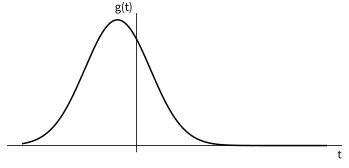
\includegraphics[width=0.8\textwidth]{fig_ch02_energy_sig.pdf} \\
                \vspace{-0.2cm} {\footnotesize (a) Signal with finite energy} \\
                \vspace{0.3cm} % (a)와 (b) 사이 간격
                
                % (b) Power Signal
                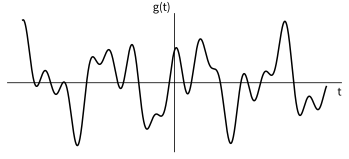
\includegraphics[width=0.8\textwidth]{fig_ch02_power_sig.pdf} \\
                \vspace{-0.2cm} {\footnotesize (b) Signal with finite power}
                
                % [통합 캡션] 맨 아래에 위치, 굵은 글씨 없음
                \caption{Examples of signals.} 
            \end{figure}
        \end{column}

        % [오른쪽 컬럼] 텍스트 설명
        \begin{column}{0.55\textwidth}
            \begin{block}{Energy Signal}
                A signal is said to be an energy signal if its energy is finite and its average power is zero.
                \[
                E = \int_{-\infty}^{\infty} |g(t)|^2 dt < \infty, \quad P = 0
                \]
            \end{block}
            %\vspace{0.1cm}
            \begin{block}{Power Signal}
                A signal is said to be a power signal if its average power is finite and its energy is infinite.
                \[
                P = \lim_{T \to \infty} \frac{1}{T} \int_{-T/2}^{T/2} |g(t)|^2 dt < \infty, \quad E = \infty
                \]
            \end{block}
        \end{column}
    \end{columns} 
\end{frame}


% Units of Signal Energy and Power
\begin{frame}{Units of Signal Power}
    \begin{itemize}
        \item The standard units of signal energy and power are the "joule" and the "watt". 
        \item However, in practice, it is often customary to use logarithmic scales to describe signal power.
        \item A signal with average power of $P$ watts has power of either $P_{dBw}$ or $P_{dBm}$.
    \end{itemize}
    
    {\centering
    \begin{columns}
        \begin{column}{0.35\textwidth}
            \begin{tcolorbox}[colframe=blue,colback=blue!5,before skip=6pt]
                $P_{dBw} = [10 \cdot \log_{10}P] \text{ dBw}$
            \end{tcolorbox}
        \end{column}
        \begin{column}{0.4\textwidth}
            \begin{tcolorbox}[colframe=red,colback=blue!5,before skip=6pt]
                $P_{dBm} = [30 + 10 \cdot \log_{10}P] \text{ dBm}$
            \end{tcolorbox}
        \end{column}
    \end{columns}
    }
    \begin{itemize}
        \item For example, \\
        \quad $P_{dBm} = -30 \text{ dBm} = 10^{-6} \text{W}$.
    \end{itemize}
\end{frame}

% Example 2.1
\begin{frame}{Example 2.1}
\begin{columns}

% [왼쪽 컬럼] 그림 (a), (b)
\begin{column}{0.3\textwidth}
\begin{figure}[h]
    \centering
    \begin{tikzpicture}[scale=0.5, >=latex]
        \colorlet{signalcolor}{green!50!black}

        % --- (a) Graph ---
        \begin{scope}[shift={(0, 3.5)}]
            % Axes
            \draw[->] (-2.5, 0) -- (5.5, 0) node[below] {$t$};
            \draw[->] (0, -0.5) -- (0, 2.5) node[right] {$g(t)$};
            
            % [수정] 원점 '0' (크기 절반)
            \node[below right, scale=0.55] at (0,0) {0};

            % [수정] Signal Waveform (진한 녹색)
            % 1. t < 0 구간 (0, 수직선, 상수 구간)
            \draw[thick, color=signalcolor] (-2.5, 0) -- (-1, 0) -- (-1, 2) -- (0, 2);
            % 2. t >= 0 구간 (지수 함수)
            \draw[thick, color=signalcolor, domain=0:5, samples=100] plot (\x, {2*exp(-\x/2)});
            
            % Label & Ticks
            \node at (2.5, 1) {$2e^{-t/2}$};
            
            % [수정] x축 눈금 숫자 (크기 절반)
            \draw (2, 0.1) -- (2, -0.1) node[below, scale=0.5] {2};
            \draw (4, 0.1) -- (4, -0.1) node[below, scale=0.5] {4};
            \draw (-1, 0.1) -- (-1, -0.1) node[below, scale=0.5] {-1};
            
            % [수정] y축 눈금 숫자 (크기 절반)
            \node[scale=0.5] at (-0.2, 2) {2};
            
            \node at (4.5, 2) {(a)};
        \end{scope}

        % --- (b) Graph ---
        \begin{scope}[shift={(0, 0)}]
            % Axes
            \draw[->] (-4.5, 0) -- (4.8, 0) node[below] {$t$};
            \draw[->] (0, -1.5) -- (0, 1.5) node[right] {$g(t)$};
            
            % [수정] 원점 '0' (크기 절반)
            \node[below right, scale=0.55] at (0,0) {0};

            % [수정] Sawtooth Wave Signal (진한 녹색)
            \foreach \x in {-3, -1, 1, 3} {
                \draw[thick, color=signalcolor] (\x, -1) -- (\x, 1); % 수직선
            }
            \foreach \x in {-5, -3, -1, 1, 3} {
                \draw[thick, color=signalcolor] (\x, -1) -- (\x+2, 1); % 빗변
            }
            
            % Dashed guide lines
            \draw[dotted, thick] (0, 1) -- (1, 1);
            \draw[dotted, thick] (0, -1) -- (-1, -1);
            
            % [수정] x축 눈금 숫자 (크기 절반)
            \foreach \x in {-4, -3, -2, -1, 1, 2, 3, 4} {
                \draw (\x, 0.1) -- (\x, -0.1) node[below, scale=0.5] {\x};
            }
            
            % [수정] y축 눈금 숫자 (크기 절반)
            \node[scale=0.5] at (0.3, 1) {1};
            \node[scale=0.5] at (0.4, -1) {-1};
            
            \node at (4, 1) {(b)};
        \end{scope}
    \end{tikzpicture}
    \caption{Signal for Example}
\end{figure}
\end{column}

\hfill

%% [오른쪽 컬럼] 문제 및 풀이
\begin{column}{0.5\textwidth}
\textbf{Problem:} Determine whether each of the following signals is an energy signal, a power signal, or neither. \\
\vspace{0.3cm}
\textbf{Solution:} \\
(a) $g(t) = \begin{cases} 2e^{-t/2}, & t \ge 0 \\ 0, & t < 0 \end{cases}$ \\
\quad Energy:
\end{column}
\end{columns}
\end{frame}





















% 3. 기본 신호 (Unit Step)
\begin{frame}{1. Basic Signals: Unit Step Function}
    \begin{columns}
        \begin{column}{0.6\textwidth}
            \centering
            % Python(ch02_signals.py)에서 생성한 그림
            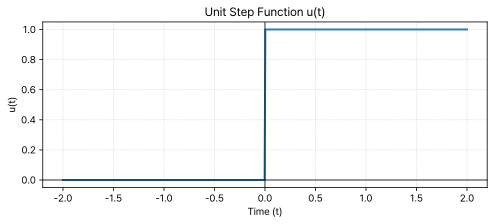
\includegraphics[width=\textwidth]{fig_ch02_unit_step.pdf}
        \end{column}
        \begin{column}{0.4\textwidth}
            \begin{block}{Definition}
                \[
                u(t) = \begin{cases} 
                1, & t \ge 0 \\ 
                0, & t < 0 
                \end{cases}
                \]
            \end{block}
            \vspace{0.2cm}
            \textbf{Key Property:} \\
            시스템의 스위칭 동작(Switching)을 수학적으로 모델링할 때 사용됨.
        \end{column}
    \end{columns}
\end{frame}

% 4. 신호의 연산 (Shifting & Scaling)
\begin{frame}{2. Signal Operations: $x(at - b)$}
    \begin{columns}
        \begin{column}{0.55\textwidth}
            \centering
            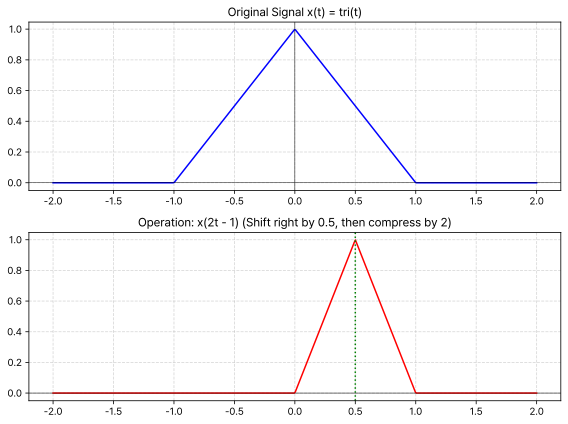
\includegraphics[width=\textwidth]{fig_ch02_operations.pdf}
        \end{column}
        \begin{column}{0.45\textwidth}
            \small
            \textbf{해석 순서 (Order of Operations):}
            \begin{enumerate}
                \item \textbf{Shifting:} $t \rightarrow t - t_0$ \\
                (Right if $t_0 > 0$)
                \item \textbf{Scaling:} $t \rightarrow at$ \\
                (Compression if $a > 1$)
            \end{enumerate}
            
            \vspace{0.3cm}
            \begin{alertblock}{Caution}
                $x(2t - 1)$은 $x(t)$를 1만큼 이동 후 2배 압축하는 것이 아님! \\
                $\rightarrow x(2(t - 0.5))$로 생각해야 함.
            \end{alertblock}
        \end{column}
    \end{columns}
\end{frame}

% 5. 상관관계 (Correlation)
\begin{frame}{3. Signal Correlation}
    \centering
    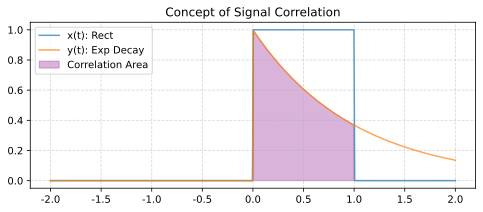
\includegraphics[width=0.7\textwidth]{fig_ch02_correlation.pdf}
    
    \vspace{0.3cm}
    \begin{block}{Correlation Coefficient ($C_n$)}
        두 신호가 얼마나 닮았는가? (Measure of Similarity)
        \[
        \rho = \frac{\int x(t) y^*(t) dt}{\sqrt{E_x E_y}}
        \]
    \end{block}
    \small \textit{그래프의 보라색 영역(Overlap)이 넓을수록 상관관계가 높습니다.}
\end{frame}

% 6. 마무리
\begin{frame}{Summary}
    \begin{itemize}
        \item \textbf{Unit Step $u(t)$:} 인과성(Causality) 표현의 핵심
        \item \textbf{Operations:} $x(at-b)$ 꼴의 변환을 자유자재로 다뤄야 함
        \item \textbf{Correlation:} 통신 시스템에서 수신 신호를 검출(Detection)하는 기본 원리
    \end{itemize}
\end{frame}

\end{document}